\documentclass{article}
\usepackage{graphicx, color}
\newcommand{\hlnumber}[1]{\textcolor[rgb]{0,0,0}{#1}}%
\newcommand{\hlfunctioncall}[1]{\textcolor[rgb]{.5,0,.33}{\textbf{#1}}}%
\newcommand{\hlstring}[1]{\textcolor[rgb]{.6,.6,1}{#1}}%
\newcommand{\hlkeyword}[1]{\textbf{#1}}%
\newcommand{\hlargument}[1]{\textcolor[rgb]{.69,.25,.02}{#1}}%
\newcommand{\hlcomment}[1]{\textcolor[rgb]{.18,.6,.34}{#1}}%
\newcommand{\hlroxygencomment}[1]{\textcolor[rgb]{.44,.48,.7}{#1}}%
\newcommand{\hlformalargs}[1]{\hlargument{#1}}%
\newcommand{\hleqformalargs}[1]{\hlargument{#1}}%
\newcommand{\hlassignement}[1]{\textbf{#1}}%
\newcommand{\hlpackage}[1]{\textcolor[rgb]{.59,.71,.145}{#1}}%
\newcommand{\hlslot}[1]{\textit{#1}}%
\newcommand{\hlsymbol}[1]{#1}%
\newcommand{\hlprompt}[1]{\textcolor[rgb]{.5,.5,.5}{#1}}%

\usepackage{color}%
 
\newsavebox{\hlnormalsizeboxclosebrace}%
\newsavebox{\hlnormalsizeboxopenbrace}%
\newsavebox{\hlnormalsizeboxbackslash}%
\newsavebox{\hlnormalsizeboxlessthan}%
\newsavebox{\hlnormalsizeboxgreaterthan}%
\newsavebox{\hlnormalsizeboxdollar}%
\newsavebox{\hlnormalsizeboxunderscore}%
\newsavebox{\hlnormalsizeboxand}%
\newsavebox{\hlnormalsizeboxhash}%
\newsavebox{\hlnormalsizeboxat}%
\newsavebox{\hlnormalsizeboxpercent}% 
\newsavebox{\hlnormalsizeboxhat}%
\newsavebox{\hlnormalsizeboxsinglequote}%
\newsavebox{\hlnormalsizeboxbacktick}%

\setbox\hlnormalsizeboxopenbrace=\hbox{\begin{normalsize}\verb.{.\end{normalsize}}%
\setbox\hlnormalsizeboxclosebrace=\hbox{\begin{normalsize}\verb.}.\end{normalsize}}%
\setbox\hlnormalsizeboxlessthan=\hbox{\begin{normalsize}\verb.<.\end{normalsize}}%
\setbox\hlnormalsizeboxdollar=\hbox{\begin{normalsize}\verb.$.\end{normalsize}}%
\setbox\hlnormalsizeboxunderscore=\hbox{\begin{normalsize}\verb._.\end{normalsize}}%
\setbox\hlnormalsizeboxand=\hbox{\begin{normalsize}\verb.&.\end{normalsize}}%
\setbox\hlnormalsizeboxhash=\hbox{\begin{normalsize}\verb.#.\end{normalsize}}%
\setbox\hlnormalsizeboxat=\hbox{\begin{normalsize}\verb.@.\end{normalsize}}%
\setbox\hlnormalsizeboxbackslash=\hbox{\begin{normalsize}\verb.\.\end{normalsize}}%
\setbox\hlnormalsizeboxgreaterthan=\hbox{\begin{normalsize}\verb.>.\end{normalsize}}%
\setbox\hlnormalsizeboxpercent=\hbox{\begin{normalsize}\verb.%.\end{normalsize}}%
\setbox\hlnormalsizeboxhat=\hbox{\begin{normalsize}\verb.^.\end{normalsize}}%
\setbox\hlnormalsizeboxsinglequote=\hbox{\begin{normalsize}\verb.'.\end{normalsize}}%
\setbox\hlnormalsizeboxbacktick=\hbox{\begin{normalsize}\verb.`.\end{normalsize}}%
\setbox\hlnormalsizeboxhat=\hbox{\begin{normalsize}\verb.^.\end{normalsize}}%



\newsavebox{\hltinyboxclosebrace}%
\newsavebox{\hltinyboxopenbrace}%
\newsavebox{\hltinyboxbackslash}%
\newsavebox{\hltinyboxlessthan}%
\newsavebox{\hltinyboxgreaterthan}%
\newsavebox{\hltinyboxdollar}%
\newsavebox{\hltinyboxunderscore}%
\newsavebox{\hltinyboxand}%
\newsavebox{\hltinyboxhash}%
\newsavebox{\hltinyboxat}%
\newsavebox{\hltinyboxpercent}% 
\newsavebox{\hltinyboxhat}%
\newsavebox{\hltinyboxsinglequote}%
\newsavebox{\hltinyboxbacktick}%

\setbox\hltinyboxopenbrace=\hbox{\begin{tiny}\verb.{.\end{tiny}}%
\setbox\hltinyboxclosebrace=\hbox{\begin{tiny}\verb.}.\end{tiny}}%
\setbox\hltinyboxlessthan=\hbox{\begin{tiny}\verb.<.\end{tiny}}%
\setbox\hltinyboxdollar=\hbox{\begin{tiny}\verb.$.\end{tiny}}%
\setbox\hltinyboxunderscore=\hbox{\begin{tiny}\verb._.\end{tiny}}%
\setbox\hltinyboxand=\hbox{\begin{tiny}\verb.&.\end{tiny}}%
\setbox\hltinyboxhash=\hbox{\begin{tiny}\verb.#.\end{tiny}}%
\setbox\hltinyboxat=\hbox{\begin{tiny}\verb.@.\end{tiny}}%
\setbox\hltinyboxbackslash=\hbox{\begin{tiny}\verb.\.\end{tiny}}%
\setbox\hltinyboxgreaterthan=\hbox{\begin{tiny}\verb.>.\end{tiny}}%
\setbox\hltinyboxpercent=\hbox{\begin{tiny}\verb.%.\end{tiny}}%
\setbox\hltinyboxhat=\hbox{\begin{tiny}\verb.^.\end{tiny}}%
\setbox\hltinyboxsinglequote=\hbox{\begin{tiny}\verb.'.\end{tiny}}%
\setbox\hltinyboxbacktick=\hbox{\begin{tiny}\verb.`.\end{tiny}}%
\setbox\hltinyboxhat=\hbox{\begin{tiny}\verb.^.\end{tiny}}%



\newsavebox{\hlscriptsizeboxclosebrace}%
\newsavebox{\hlscriptsizeboxopenbrace}%
\newsavebox{\hlscriptsizeboxbackslash}%
\newsavebox{\hlscriptsizeboxlessthan}%
\newsavebox{\hlscriptsizeboxgreaterthan}%
\newsavebox{\hlscriptsizeboxdollar}%
\newsavebox{\hlscriptsizeboxunderscore}%
\newsavebox{\hlscriptsizeboxand}%
\newsavebox{\hlscriptsizeboxhash}%
\newsavebox{\hlscriptsizeboxat}%
\newsavebox{\hlscriptsizeboxpercent}% 
\newsavebox{\hlscriptsizeboxhat}%
\newsavebox{\hlscriptsizeboxsinglequote}%
\newsavebox{\hlscriptsizeboxbacktick}%

\setbox\hlscriptsizeboxopenbrace=\hbox{\begin{scriptsize}\verb.{.\end{scriptsize}}%
\setbox\hlscriptsizeboxclosebrace=\hbox{\begin{scriptsize}\verb.}.\end{scriptsize}}%
\setbox\hlscriptsizeboxlessthan=\hbox{\begin{scriptsize}\verb.<.\end{scriptsize}}%
\setbox\hlscriptsizeboxdollar=\hbox{\begin{scriptsize}\verb.$.\end{scriptsize}}%
\setbox\hlscriptsizeboxunderscore=\hbox{\begin{scriptsize}\verb._.\end{scriptsize}}%
\setbox\hlscriptsizeboxand=\hbox{\begin{scriptsize}\verb.&.\end{scriptsize}}%
\setbox\hlscriptsizeboxhash=\hbox{\begin{scriptsize}\verb.#.\end{scriptsize}}%
\setbox\hlscriptsizeboxat=\hbox{\begin{scriptsize}\verb.@.\end{scriptsize}}%
\setbox\hlscriptsizeboxbackslash=\hbox{\begin{scriptsize}\verb.\.\end{scriptsize}}%
\setbox\hlscriptsizeboxgreaterthan=\hbox{\begin{scriptsize}\verb.>.\end{scriptsize}}%
\setbox\hlscriptsizeboxpercent=\hbox{\begin{scriptsize}\verb.%.\end{scriptsize}}%
\setbox\hlscriptsizeboxhat=\hbox{\begin{scriptsize}\verb.^.\end{scriptsize}}%
\setbox\hlscriptsizeboxsinglequote=\hbox{\begin{scriptsize}\verb.'.\end{scriptsize}}%
\setbox\hlscriptsizeboxbacktick=\hbox{\begin{scriptsize}\verb.`.\end{scriptsize}}%
\setbox\hlscriptsizeboxhat=\hbox{\begin{scriptsize}\verb.^.\end{scriptsize}}%



\newsavebox{\hlfootnotesizeboxclosebrace}%
\newsavebox{\hlfootnotesizeboxopenbrace}%
\newsavebox{\hlfootnotesizeboxbackslash}%
\newsavebox{\hlfootnotesizeboxlessthan}%
\newsavebox{\hlfootnotesizeboxgreaterthan}%
\newsavebox{\hlfootnotesizeboxdollar}%
\newsavebox{\hlfootnotesizeboxunderscore}%
\newsavebox{\hlfootnotesizeboxand}%
\newsavebox{\hlfootnotesizeboxhash}%
\newsavebox{\hlfootnotesizeboxat}%
\newsavebox{\hlfootnotesizeboxpercent}% 
\newsavebox{\hlfootnotesizeboxhat}%
\newsavebox{\hlfootnotesizeboxsinglequote}%
\newsavebox{\hlfootnotesizeboxbacktick}%

\setbox\hlfootnotesizeboxopenbrace=\hbox{\begin{footnotesize}\verb.{.\end{footnotesize}}%
\setbox\hlfootnotesizeboxclosebrace=\hbox{\begin{footnotesize}\verb.}.\end{footnotesize}}%
\setbox\hlfootnotesizeboxlessthan=\hbox{\begin{footnotesize}\verb.<.\end{footnotesize}}%
\setbox\hlfootnotesizeboxdollar=\hbox{\begin{footnotesize}\verb.$.\end{footnotesize}}%
\setbox\hlfootnotesizeboxunderscore=\hbox{\begin{footnotesize}\verb._.\end{footnotesize}}%
\setbox\hlfootnotesizeboxand=\hbox{\begin{footnotesize}\verb.&.\end{footnotesize}}%
\setbox\hlfootnotesizeboxhash=\hbox{\begin{footnotesize}\verb.#.\end{footnotesize}}%
\setbox\hlfootnotesizeboxat=\hbox{\begin{footnotesize}\verb.@.\end{footnotesize}}%
\setbox\hlfootnotesizeboxbackslash=\hbox{\begin{footnotesize}\verb.\.\end{footnotesize}}%
\setbox\hlfootnotesizeboxgreaterthan=\hbox{\begin{footnotesize}\verb.>.\end{footnotesize}}%
\setbox\hlfootnotesizeboxpercent=\hbox{\begin{footnotesize}\verb.%.\end{footnotesize}}%
\setbox\hlfootnotesizeboxhat=\hbox{\begin{footnotesize}\verb.^.\end{footnotesize}}%
\setbox\hlfootnotesizeboxsinglequote=\hbox{\begin{footnotesize}\verb.'.\end{footnotesize}}%
\setbox\hlfootnotesizeboxbacktick=\hbox{\begin{footnotesize}\verb.`.\end{footnotesize}}%
\setbox\hlfootnotesizeboxhat=\hbox{\begin{footnotesize}\verb.^.\end{footnotesize}}%



\newsavebox{\hlsmallboxclosebrace}%
\newsavebox{\hlsmallboxopenbrace}%
\newsavebox{\hlsmallboxbackslash}%
\newsavebox{\hlsmallboxlessthan}%
\newsavebox{\hlsmallboxgreaterthan}%
\newsavebox{\hlsmallboxdollar}%
\newsavebox{\hlsmallboxunderscore}%
\newsavebox{\hlsmallboxand}%
\newsavebox{\hlsmallboxhash}%
\newsavebox{\hlsmallboxat}%
\newsavebox{\hlsmallboxpercent}% 
\newsavebox{\hlsmallboxhat}%
\newsavebox{\hlsmallboxsinglequote}%
\newsavebox{\hlsmallboxbacktick}%

\setbox\hlsmallboxopenbrace=\hbox{\begin{small}\verb.{.\end{small}}%
\setbox\hlsmallboxclosebrace=\hbox{\begin{small}\verb.}.\end{small}}%
\setbox\hlsmallboxlessthan=\hbox{\begin{small}\verb.<.\end{small}}%
\setbox\hlsmallboxdollar=\hbox{\begin{small}\verb.$.\end{small}}%
\setbox\hlsmallboxunderscore=\hbox{\begin{small}\verb._.\end{small}}%
\setbox\hlsmallboxand=\hbox{\begin{small}\verb.&.\end{small}}%
\setbox\hlsmallboxhash=\hbox{\begin{small}\verb.#.\end{small}}%
\setbox\hlsmallboxat=\hbox{\begin{small}\verb.@.\end{small}}%
\setbox\hlsmallboxbackslash=\hbox{\begin{small}\verb.\.\end{small}}%
\setbox\hlsmallboxgreaterthan=\hbox{\begin{small}\verb.>.\end{small}}%
\setbox\hlsmallboxpercent=\hbox{\begin{small}\verb.%.\end{small}}%
\setbox\hlsmallboxhat=\hbox{\begin{small}\verb.^.\end{small}}%
\setbox\hlsmallboxsinglequote=\hbox{\begin{small}\verb.'.\end{small}}%
\setbox\hlsmallboxbacktick=\hbox{\begin{small}\verb.`.\end{small}}%
\setbox\hlsmallboxhat=\hbox{\begin{small}\verb.^.\end{small}}%



\newsavebox{\hllargeboxclosebrace}%
\newsavebox{\hllargeboxopenbrace}%
\newsavebox{\hllargeboxbackslash}%
\newsavebox{\hllargeboxlessthan}%
\newsavebox{\hllargeboxgreaterthan}%
\newsavebox{\hllargeboxdollar}%
\newsavebox{\hllargeboxunderscore}%
\newsavebox{\hllargeboxand}%
\newsavebox{\hllargeboxhash}%
\newsavebox{\hllargeboxat}%
\newsavebox{\hllargeboxpercent}% 
\newsavebox{\hllargeboxhat}%
\newsavebox{\hllargeboxsinglequote}%
\newsavebox{\hllargeboxbacktick}%

\setbox\hllargeboxopenbrace=\hbox{\begin{large}\verb.{.\end{large}}%
\setbox\hllargeboxclosebrace=\hbox{\begin{large}\verb.}.\end{large}}%
\setbox\hllargeboxlessthan=\hbox{\begin{large}\verb.<.\end{large}}%
\setbox\hllargeboxdollar=\hbox{\begin{large}\verb.$.\end{large}}%
\setbox\hllargeboxunderscore=\hbox{\begin{large}\verb._.\end{large}}%
\setbox\hllargeboxand=\hbox{\begin{large}\verb.&.\end{large}}%
\setbox\hllargeboxhash=\hbox{\begin{large}\verb.#.\end{large}}%
\setbox\hllargeboxat=\hbox{\begin{large}\verb.@.\end{large}}%
\setbox\hllargeboxbackslash=\hbox{\begin{large}\verb.\.\end{large}}%
\setbox\hllargeboxgreaterthan=\hbox{\begin{large}\verb.>.\end{large}}%
\setbox\hllargeboxpercent=\hbox{\begin{large}\verb.%.\end{large}}%
\setbox\hllargeboxhat=\hbox{\begin{large}\verb.^.\end{large}}%
\setbox\hllargeboxsinglequote=\hbox{\begin{large}\verb.'.\end{large}}%
\setbox\hllargeboxbacktick=\hbox{\begin{large}\verb.`.\end{large}}%
\setbox\hllargeboxhat=\hbox{\begin{large}\verb.^.\end{large}}%



\newsavebox{\hlLargeboxclosebrace}%
\newsavebox{\hlLargeboxopenbrace}%
\newsavebox{\hlLargeboxbackslash}%
\newsavebox{\hlLargeboxlessthan}%
\newsavebox{\hlLargeboxgreaterthan}%
\newsavebox{\hlLargeboxdollar}%
\newsavebox{\hlLargeboxunderscore}%
\newsavebox{\hlLargeboxand}%
\newsavebox{\hlLargeboxhash}%
\newsavebox{\hlLargeboxat}%
\newsavebox{\hlLargeboxpercent}% 
\newsavebox{\hlLargeboxhat}%
\newsavebox{\hlLargeboxsinglequote}%
\newsavebox{\hlLargeboxbacktick}%

\setbox\hlLargeboxopenbrace=\hbox{\begin{Large}\verb.{.\end{Large}}%
\setbox\hlLargeboxclosebrace=\hbox{\begin{Large}\verb.}.\end{Large}}%
\setbox\hlLargeboxlessthan=\hbox{\begin{Large}\verb.<.\end{Large}}%
\setbox\hlLargeboxdollar=\hbox{\begin{Large}\verb.$.\end{Large}}%
\setbox\hlLargeboxunderscore=\hbox{\begin{Large}\verb._.\end{Large}}%
\setbox\hlLargeboxand=\hbox{\begin{Large}\verb.&.\end{Large}}%
\setbox\hlLargeboxhash=\hbox{\begin{Large}\verb.#.\end{Large}}%
\setbox\hlLargeboxat=\hbox{\begin{Large}\verb.@.\end{Large}}%
\setbox\hlLargeboxbackslash=\hbox{\begin{Large}\verb.\.\end{Large}}%
\setbox\hlLargeboxgreaterthan=\hbox{\begin{Large}\verb.>.\end{Large}}%
\setbox\hlLargeboxpercent=\hbox{\begin{Large}\verb.%.\end{Large}}%
\setbox\hlLargeboxhat=\hbox{\begin{Large}\verb.^.\end{Large}}%
\setbox\hlLargeboxsinglequote=\hbox{\begin{Large}\verb.'.\end{Large}}%
\setbox\hlLargeboxbacktick=\hbox{\begin{Large}\verb.`.\end{Large}}%
\setbox\hlLargeboxhat=\hbox{\begin{Large}\verb.^.\end{Large}}%



\newsavebox{\hlLARGEboxclosebrace}%
\newsavebox{\hlLARGEboxopenbrace}%
\newsavebox{\hlLARGEboxbackslash}%
\newsavebox{\hlLARGEboxlessthan}%
\newsavebox{\hlLARGEboxgreaterthan}%
\newsavebox{\hlLARGEboxdollar}%
\newsavebox{\hlLARGEboxunderscore}%
\newsavebox{\hlLARGEboxand}%
\newsavebox{\hlLARGEboxhash}%
\newsavebox{\hlLARGEboxat}%
\newsavebox{\hlLARGEboxpercent}% 
\newsavebox{\hlLARGEboxhat}%
\newsavebox{\hlLARGEboxsinglequote}%
\newsavebox{\hlLARGEboxbacktick}%

\setbox\hlLARGEboxopenbrace=\hbox{\begin{LARGE}\verb.{.\end{LARGE}}%
\setbox\hlLARGEboxclosebrace=\hbox{\begin{LARGE}\verb.}.\end{LARGE}}%
\setbox\hlLARGEboxlessthan=\hbox{\begin{LARGE}\verb.<.\end{LARGE}}%
\setbox\hlLARGEboxdollar=\hbox{\begin{LARGE}\verb.$.\end{LARGE}}%
\setbox\hlLARGEboxunderscore=\hbox{\begin{LARGE}\verb._.\end{LARGE}}%
\setbox\hlLARGEboxand=\hbox{\begin{LARGE}\verb.&.\end{LARGE}}%
\setbox\hlLARGEboxhash=\hbox{\begin{LARGE}\verb.#.\end{LARGE}}%
\setbox\hlLARGEboxat=\hbox{\begin{LARGE}\verb.@.\end{LARGE}}%
\setbox\hlLARGEboxbackslash=\hbox{\begin{LARGE}\verb.\.\end{LARGE}}%
\setbox\hlLARGEboxgreaterthan=\hbox{\begin{LARGE}\verb.>.\end{LARGE}}%
\setbox\hlLARGEboxpercent=\hbox{\begin{LARGE}\verb.%.\end{LARGE}}%
\setbox\hlLARGEboxhat=\hbox{\begin{LARGE}\verb.^.\end{LARGE}}%
\setbox\hlLARGEboxsinglequote=\hbox{\begin{LARGE}\verb.'.\end{LARGE}}%
\setbox\hlLARGEboxbacktick=\hbox{\begin{LARGE}\verb.`.\end{LARGE}}%
\setbox\hlLARGEboxhat=\hbox{\begin{LARGE}\verb.^.\end{LARGE}}%



\newsavebox{\hlhugeboxclosebrace}%
\newsavebox{\hlhugeboxopenbrace}%
\newsavebox{\hlhugeboxbackslash}%
\newsavebox{\hlhugeboxlessthan}%
\newsavebox{\hlhugeboxgreaterthan}%
\newsavebox{\hlhugeboxdollar}%
\newsavebox{\hlhugeboxunderscore}%
\newsavebox{\hlhugeboxand}%
\newsavebox{\hlhugeboxhash}%
\newsavebox{\hlhugeboxat}%
\newsavebox{\hlhugeboxpercent}% 
\newsavebox{\hlhugeboxhat}%
\newsavebox{\hlhugeboxsinglequote}%
\newsavebox{\hlhugeboxbacktick}%

\setbox\hlhugeboxopenbrace=\hbox{\begin{huge}\verb.{.\end{huge}}%
\setbox\hlhugeboxclosebrace=\hbox{\begin{huge}\verb.}.\end{huge}}%
\setbox\hlhugeboxlessthan=\hbox{\begin{huge}\verb.<.\end{huge}}%
\setbox\hlhugeboxdollar=\hbox{\begin{huge}\verb.$.\end{huge}}%
\setbox\hlhugeboxunderscore=\hbox{\begin{huge}\verb._.\end{huge}}%
\setbox\hlhugeboxand=\hbox{\begin{huge}\verb.&.\end{huge}}%
\setbox\hlhugeboxhash=\hbox{\begin{huge}\verb.#.\end{huge}}%
\setbox\hlhugeboxat=\hbox{\begin{huge}\verb.@.\end{huge}}%
\setbox\hlhugeboxbackslash=\hbox{\begin{huge}\verb.\.\end{huge}}%
\setbox\hlhugeboxgreaterthan=\hbox{\begin{huge}\verb.>.\end{huge}}%
\setbox\hlhugeboxpercent=\hbox{\begin{huge}\verb.%.\end{huge}}%
\setbox\hlhugeboxhat=\hbox{\begin{huge}\verb.^.\end{huge}}%
\setbox\hlhugeboxsinglequote=\hbox{\begin{huge}\verb.'.\end{huge}}%
\setbox\hlhugeboxbacktick=\hbox{\begin{huge}\verb.`.\end{huge}}%
\setbox\hlhugeboxhat=\hbox{\begin{huge}\verb.^.\end{huge}}%



\newsavebox{\hlHugeboxclosebrace}%
\newsavebox{\hlHugeboxopenbrace}%
\newsavebox{\hlHugeboxbackslash}%
\newsavebox{\hlHugeboxlessthan}%
\newsavebox{\hlHugeboxgreaterthan}%
\newsavebox{\hlHugeboxdollar}%
\newsavebox{\hlHugeboxunderscore}%
\newsavebox{\hlHugeboxand}%
\newsavebox{\hlHugeboxhash}%
\newsavebox{\hlHugeboxat}%
\newsavebox{\hlHugeboxpercent}% 
\newsavebox{\hlHugeboxhat}%
\newsavebox{\hlHugeboxsinglequote}%
\newsavebox{\hlHugeboxbacktick}%

\setbox\hlHugeboxopenbrace=\hbox{\begin{Huge}\verb.{.\end{Huge}}%
\setbox\hlHugeboxclosebrace=\hbox{\begin{Huge}\verb.}.\end{Huge}}%
\setbox\hlHugeboxlessthan=\hbox{\begin{Huge}\verb.<.\end{Huge}}%
\setbox\hlHugeboxdollar=\hbox{\begin{Huge}\verb.$.\end{Huge}}%
\setbox\hlHugeboxunderscore=\hbox{\begin{Huge}\verb._.\end{Huge}}%
\setbox\hlHugeboxand=\hbox{\begin{Huge}\verb.&.\end{Huge}}%
\setbox\hlHugeboxhash=\hbox{\begin{Huge}\verb.#.\end{Huge}}%
\setbox\hlHugeboxat=\hbox{\begin{Huge}\verb.@.\end{Huge}}%
\setbox\hlHugeboxbackslash=\hbox{\begin{Huge}\verb.\.\end{Huge}}%
\setbox\hlHugeboxgreaterthan=\hbox{\begin{Huge}\verb.>.\end{Huge}}%
\setbox\hlHugeboxpercent=\hbox{\begin{Huge}\verb.%.\end{Huge}}%
\setbox\hlHugeboxhat=\hbox{\begin{Huge}\verb.^.\end{Huge}}%
\setbox\hlHugeboxsinglequote=\hbox{\begin{Huge}\verb.'.\end{Huge}}%
\setbox\hlHugeboxbacktick=\hbox{\begin{Huge}\verb.`.\end{Huge}}%
\setbox\hlHugeboxhat=\hbox{\begin{Huge}\verb.^.\end{Huge}}%
 

\def\urltilda{\kern -.15em\lower .7ex\hbox{\~{}}\kern .04em}%

\newcommand{\hlstd}[1]{\textcolor[rgb]{0,0,0}{#1}}%
\newcommand{\hlnum}[1]{\textcolor[rgb]{0.16,0.16,1}{#1}}
\newcommand{\hlesc}[1]{\textcolor[rgb]{1,0,1}{#1}}
\newcommand{\hlstr}[1]{\textcolor[rgb]{1,0,0}{#1}}
\newcommand{\hldstr}[1]{\textcolor[rgb]{0.51,0.51,0}{#1}}
\newcommand{\hlslc}[1]{\textcolor[rgb]{0.51,0.51,0.51}{\it{#1}}}
\newcommand{\hlcom}[1]{\textcolor[rgb]{0.51,0.51,0.51}{\it{#1}}}
\newcommand{\hldir}[1]{\textcolor[rgb]{0,0.51,0}{#1}}
\newcommand{\hlsym}[1]{\textcolor[rgb]{0,0,0}{#1}}
\newcommand{\hlline}[1]{\textcolor[rgb]{0.33,0.33,0.33}{#1}}
\newcommand{\hlkwa}[1]{\textcolor[rgb]{0,0,0}{\bf{#1}}}
\newcommand{\hlkwb}[1]{\textcolor[rgb]{0.51,0,0}{#1}}
\newcommand{\hlkwc}[1]{\textcolor[rgb]{0,0,0}{\bf{#1}}}
\newcommand{\hlkwd}[1]{\textcolor[rgb]{0,0,0.51}{#1}}

\definecolor{fgcolor}{rgb}{0,0,0}
\usepackage{framed}
\makeatletter
\newenvironment{kframe}{%
 \def\FrameCommand##1{\hskip\@totalleftmargin \hskip-\fboxsep
 \colorbox{shadecolor}{##1}\hskip-\fboxsep
     % There is no \@totalrightmargin, so:
     \hskip-\linewidth \hskip-\@totalleftmargin \hskip\columnwidth}%
 \MakeFramed {\advance\hsize-\width
   \@totalleftmargin\z@ \linewidth\hsize
   \@setminipage}}%
 {\par\unskip\endMakeFramed}
\makeatother

\newenvironment{knitrout}{}{} % an empty environment to be redefined in TeX

\usepackage[sc]{mathpazo}
\usepackage[T1]{fontenc}
\usepackage{geometry}
\usepackage{amssymb}
\usepackage{amsmath}
\geometry{verbose,tmargin=2.5cm,bmargin=2.5cm,lmargin=2.5cm,rmargin=2.5cm}
\setcounter{secnumdepth}{2}
\setcounter{tocdepth}{2}
\usepackage{url}
\usepackage[unicode=true,pdfusetitle,
 bookmarks=true,bookmarksnumbered=true,bookmarksopen=true,bookmarksopenlevel=2,
 breaklinks=false,pdfborder={0 0 1},backref=false,colorlinks=false]
 {hyperref}
\hypersetup{
 pdfstartview={XYZ null null 1}}
%\usepackage{breakurl}

\makeatletter
%%%%%%%%%%%%%%%%%%%%%%%%%%%%%% User specified LaTeX commands.
\renewcommand{\textfraction}{0.05}
\renewcommand{\topfraction}{0.8}
\renewcommand{\bottomfraction}{0.8}
\renewcommand{\floatpagefraction}{0.75}

\makeatother

\begin{document}

%% still can't get paths to work ...





\begin{center}
  {\bf \Large Homework 9, Statistical Rethinking}\\
\vspace{12pt}
   {\large Jaime Ashander}
\end{center}

\subsection*{Contraception in Bangladesh}

Looking at fertility in Bangladesh circa 1980. 

\begin{knitrout}
\definecolor{shadecolor}{rgb}{.97, .97, .97}{\color{fgcolor}\begin{kframe}
\begin{flushleft}
\ttfamily\noindent
\hlsymbol{d}{\ }\hlassignement{\usebox{\hlnormalsizeboxlessthan}-}{\ }\hlfunctioncall{read.csv}\hlkeyword{(}\hlstring{"bangladesh.csv"}\hlkeyword{)}\hspace*{\fill}\\
\hlstd{}\hlfunctioncall{head}\hlkeyword{(}\hlsymbol{d}\hlkeyword{,}{\ }\hlargument{n}{\ }\hlargument{=}{\ }\hlnumber{1}\hlkeyword{)}\mbox{}
\normalfont
\end{flushleft}
\begin{verbatim}
##   woman district use.contraception living.children age.centered urban
## 1     1        1                 0               4        18.44     1
\end{verbatim}
\begin{flushleft}
\ttfamily\noindent
\hlsymbol{dist.pop}{\ }\hlassignement{\usebox{\hlnormalsizeboxlessthan}-}{\ }\hlfunctioncall{table}\hlkeyword{(}\hlsymbol{d}\hlkeyword{\usebox{\hlnormalsizeboxdollar}}\hlsymbol{district}\hlkeyword{)}{\ }{\ }\hlcomment{\usebox{\hlnormalsizeboxhash}\usebox{\hlnormalsizeboxhash}{\ }population{\ }column}\hspace*{\fill}\\
\hlstd{}\hlsymbol{d}\hlkeyword{\usebox{\hlnormalsizeboxdollar}}\hlsymbol{population}{\ }\hlassignement{\usebox{\hlnormalsizeboxlessthan}-}{\ }\hlfunctioncall{sapply}\hlkeyword{(}\hlsymbol{d}\hlkeyword{\usebox{\hlnormalsizeboxdollar}}\hlsymbol{district}\hlkeyword{,}{\ }\hlkeyword{function}\hlkeyword{(}\hlformalargs{i}\hlkeyword{)}{\ }\hlsymbol{dist.pop}\hlkeyword{[}\hlfunctioncall{match}\hlkeyword{(}\hlsymbol{i}\hlkeyword{,}\hspace*{\fill}\\
\hlstd{}{\ }{\ }{\ }{\ }\hlfunctioncall{row.names}\hlkeyword{(}\hlsymbol{dist.pop}\hlkeyword{)}\hlkeyword{)}\hlkeyword{]}\hlkeyword{)}\mbox{}
\normalfont
\end{flushleft}
\end{kframe}}
\end{knitrout}


I'm modelling {\tt use.contraception} indicating contraception use, with predictor variables {\tt district}, defining the woman's location in political geography of Bangladesh, and {\tt urban} indicating city or rural.

\subsection*{Predicting contraception use}


First, I will model contraception use accounting for clustering of observations by district. 
I'll compare a model with a fixed effect for {\tt district} with a mixed effects model that puts random effects on {\tt district}

\begin{knitrout}
\definecolor{shadecolor}{rgb}{.97, .97, .97}{\color{fgcolor}\begin{kframe}
\begin{flushleft}
\ttfamily\noindent
\hlsymbol{m1}{\ }\hlassignement{\usebox{\hlnormalsizeboxlessthan}-}{\ }\hlfunctioncall{glm}\hlkeyword{(}\hlsymbol{use.contraception}{\ }\hlkeyword{\urltilda{}}{\ }\hlfunctioncall{as.factor}\hlkeyword{(}\hlsymbol{district}\hlkeyword{)}\hlkeyword{,}{\ }\hlargument{data}{\ }\hlargument{=}{\ }\hlsymbol{d}\hlkeyword{,}\hspace*{\fill}\\
\hlstd{}{\ }{\ }{\ }{\ }\hlargument{family}{\ }\hlargument{=}{\ }\hlsymbol{binomial}\hlkeyword{)}\hspace*{\fill}\\
\hlstd{}\hlsymbol{m2}{\ }\hlassignement{\usebox{\hlnormalsizeboxlessthan}-}{\ }\hlfunctioncall{glmer}\hlkeyword{(}\hlsymbol{use.contraception}{\ }\hlkeyword{\urltilda{}}{\ }\hlkeyword{(}\hlnumber{1}{\ }\hlkeyword{|}{\ }\hlsymbol{district}\hlkeyword{)}\hlkeyword{,}{\ }\hlargument{data}{\ }\hlargument{=}{\ }\hlsymbol{d}\hlkeyword{,}\hspace*{\fill}\\
\hlstd{}{\ }{\ }{\ }{\ }\hlargument{family}{\ }\hlargument{=}{\ }\hlsymbol{binomial}\hlkeyword{)}\hspace*{\fill}\\
\hlstd{}\hlfunctioncall{precis}\hlkeyword{(}\hlsymbol{m2}\hlkeyword{)}\mbox{}
\normalfont
\end{flushleft}
\begin{verbatim}
##                        Estimate Std. Error    2.5%   97.5%
## (Intercept)             -0.5379    0.08395 -0.7024 -0.3733
## ((Intercept)|district)   0.4957         NA      NA      NA
\end{verbatim}
\end{kframe}}
\end{knitrout}


\subsubsection*{Mixed effects or not?}


\begin{knitrout}
\definecolor{shadecolor}{rgb}{.97, .97, .97}{\color{fgcolor}\begin{kframe}
\begin{flushleft}
\ttfamily\noindent
\hlsymbol{d2}{\ }\hlassignement{\usebox{\hlnormalsizeboxlessthan}-}{\ }\hlfunctioncall{fortify}\hlkeyword{(}\hlsymbol{m1}\hlkeyword{,}{\ }\hlsymbol{d}\hlkeyword{)}{\ }{\ }\hlcomment{\usebox{\hlnormalsizeboxhash}add{\ }predictions{\ }to{\ }data{\ }logistic(d2\usebox{\hlnormalsizeboxdollar}.fitted){\ }gives{\ }predictions}\hspace*{\fill}\\
\hlstd{}\hlsymbol{d2}\hlkeyword{\usebox{\hlnormalsizeboxdollar}}\hlsymbol{upper}{\ }\hlassignement{\usebox{\hlnormalsizeboxlessthan}-}{\ }\hlfunctioncall{with}\hlkeyword{(}\hlsymbol{d2}\hlkeyword{,}{\ }\hlfunctioncall{ifelse}\hlkeyword{(}\hlsymbol{population}{\ }\hlkeyword{\usebox{\hlnormalsizeboxgreaterthan}}{\ }\hlfunctioncall{median}\hlkeyword{(}\hlfunctioncall{unique}\hlkeyword{(}\hlsymbol{population}\hlkeyword{)}\hlkeyword{)}\hlkeyword{,}\hspace*{\fill}\\
\hlstd{}{\ }{\ }{\ }{\ }\hlnumber{FALSE}\hlkeyword{,}{\ }\hlnumber{TRUE}\hlkeyword{)}\hlkeyword{)}\hspace*{\fill}\\
\hlstd{}\hlsymbol{d2}\hlkeyword{\usebox{\hlnormalsizeboxdollar}}\hlsymbol{m1}{\ }\hlassignement{\usebox{\hlnormalsizeboxlessthan}-}{\ }\hlfunctioncall{logistic}\hlkeyword{(}\hlsymbol{d2}\hlkeyword{\usebox{\hlnormalsizeboxdollar}}\hlsymbol{.fitted}\hlkeyword{)}\hspace*{\fill}\\
\hlstd{}\hspace*{\fill}\\
\hlstd{}\hlsymbol{re2}{\ }\hlassignement{\usebox{\hlnormalsizeboxlessthan}-}{\ }\hlfunctioncall{ranef}\hlkeyword{(}\hlsymbol{m2}\hlkeyword{)}\hlkeyword{\usebox{\hlnormalsizeboxdollar}}\hlsymbol{district}\hspace*{\fill}\\
\hlstd{}\hlsymbol{fe2}{\ }\hlassignement{\usebox{\hlnormalsizeboxlessthan}-}{\ }\hlfunctioncall{fixef}\hlkeyword{(}\hlsymbol{m2}\hlkeyword{)}\hspace*{\fill}\\
\hlstd{}\hlsymbol{d2}\hlkeyword{\usebox{\hlnormalsizeboxdollar}}\hlsymbol{m2}{\ }\hlassignement{\usebox{\hlnormalsizeboxlessthan}-}{\ }\hlfunctioncall{sapply}\hlkeyword{(}\hlsymbol{d2}\hlkeyword{\usebox{\hlnormalsizeboxdollar}}\hlsymbol{district}\hlkeyword{,}{\ }\hlkeyword{function}\hlkeyword{(}\hlformalargs{i}\hlkeyword{)}{\ }\hlfunctioncall{logistic}\hlkeyword{(}\hlsymbol{fe2}{\ }\hlkeyword{+}{\ }\hlsymbol{re2}\hlkeyword{[}\hlfunctioncall{match}\hlkeyword{(}\hlsymbol{i}\hlkeyword{,}\hspace*{\fill}\\
\hlstd{}{\ }{\ }{\ }{\ }\hlfunctioncall{row.names}\hlkeyword{(}\hlsymbol{re2}\hlkeyword{)}\hlkeyword{)}\hlkeyword{,}{\ }\hlkeyword{]}\hlkeyword{)}\hlkeyword{)}\hspace*{\fill}\\
\hlstd{}\hspace*{\fill}\\
\hlstd{}\hlsymbol{d2}\hlkeyword{\usebox{\hlnormalsizeboxdollar}}\hlsymbol{District}{\ }\hlassignement{\usebox{\hlnormalsizeboxlessthan}-}{\ }\hlfunctioncall{with}\hlkeyword{(}\hlsymbol{d2}\hlkeyword{,}{\ }\hlfunctioncall{factor}\hlkeyword{(}\hlsymbol{district}\hlkeyword{,}{\ }\hlargument{levels}{\ }\hlargument{=}{\ }\hlfunctioncall{unique}\hlkeyword{(}\hlsymbol{district}\hlkeyword{[}\hlfunctioncall{order}\hlkeyword{(}\hlsymbol{population}\hlkeyword{)}\hlkeyword{]}\hlkeyword{)}\hlkeyword{)}\hlkeyword{)}\hspace*{\fill}\\
\hlstd{}\hspace*{\fill}\\
\hlstd{}\hlsymbol{g}{\ }\hlassignement{\usebox{\hlnormalsizeboxlessthan}-}{\ }\hlfunctioncall{ggplot}\hlkeyword{(}\hlfunctioncall{subset}\hlkeyword{(}\hlsymbol{d2}\hlkeyword{,}{\ }\hlsymbol{upper}\hlkeyword{)}\hlkeyword{)}{\ }\hlkeyword{+}{\ }\hlfunctioncall{theme\usebox{\hlnormalsizeboxunderscore}bw}\hlkeyword{(}\hlkeyword{)}\hspace*{\fill}\\
\hlstd{}\hlsymbol{g}{\ }\hlassignement{\usebox{\hlnormalsizeboxlessthan}-}{\ }\hlsymbol{g}{\ }\hlkeyword{+}{\ }\hlfunctioncall{geom\usebox{\hlnormalsizeboxunderscore}violin}\hlkeyword{(}\hlfunctioncall{aes}\hlkeyword{(}\hlsymbol{District}\hlkeyword{,}{\ }\hlsymbol{use.contraception}\hlkeyword{)}\hlkeyword{,}{\ }\hlargument{alpha}{\ }\hlargument{=}{\ }\hlnumber{0.5}\hlkeyword{,}\hspace*{\fill}\\
\hlstd{}{\ }{\ }{\ }{\ }\hlargument{fill}{\ }\hlargument{=}{\ }\hlstring{"lightgrey"}\hlkeyword{,}{\ }\hlargument{color}{\ }\hlargument{=}{\ }\hlstring{"lightgray"}\hlkeyword{)}{\ }{\ }\hlcomment{\usebox{\hlnormalsizeboxhash}\usebox{\hlnormalsizeboxhash}{\ }construct{\ }a{\ }violin{\ }plot{\ }for{\ }use/non-use{\ }each{\ }district}\hspace*{\fill}\\
\hlstd{}\hlsymbol{g}{\ }\hlassignement{\usebox{\hlnormalsizeboxlessthan}-}{\ }\hlsymbol{g}{\ }\hlkeyword{+}{\ }\hlfunctioncall{geom\usebox{\hlnormalsizeboxunderscore}point}\hlkeyword{(}\hlfunctioncall{aes}\hlkeyword{(}\hlsymbol{District}\hlkeyword{,}{\ }\hlsymbol{m1}\hlkeyword{)}\hlkeyword{,}{\ }\hlargument{size}{\ }\hlargument{=}{\ }\hlnumber{1.5}\hlkeyword{)}\hspace*{\fill}\\
\hlstd{}\hlsymbol{g}{\ }\hlassignement{\usebox{\hlnormalsizeboxlessthan}-}{\ }\hlsymbol{g}{\ }\hlkeyword{+}{\ }\hlfunctioncall{geom\usebox{\hlnormalsizeboxunderscore}point}\hlkeyword{(}\hlfunctioncall{aes}\hlkeyword{(}\hlsymbol{District}\hlkeyword{,}{\ }\hlsymbol{m2}\hlkeyword{)}\hlkeyword{,}{\ }\hlargument{color}{\ }\hlargument{=}{\ }\hlstring{"darkgrey"}\hlkeyword{,}\hspace*{\fill}\\
\hlstd{}{\ }{\ }{\ }{\ }\hlargument{size}{\ }\hlargument{=}{\ }\hlnumber{2}\hlkeyword{)}{\ }\hlkeyword{+}{\ }\hlfunctioncall{geom\usebox{\hlnormalsizeboxunderscore}hline}\hlkeyword{(}\hlargument{yintercept}{\ }\hlargument{=}{\ }\hlfunctioncall{logistic}\hlkeyword{(}\hlsymbol{fe2}\hlkeyword{)}\hlkeyword{,}{\ }\hlargument{color}{\ }\hlargument{=}{\ }\hlstring{"darkgrey"}\hlkeyword{,}\hspace*{\fill}\\
\hlstd{}{\ }{\ }{\ }{\ }\hlargument{linetype}{\ }\hlargument{=}{\ }\hlnumber{2}\hlkeyword{)}\hspace*{\fill}\\
\hlstd{}\hlsymbol{g1}{\ }\hlassignement{\usebox{\hlnormalsizeboxlessthan}-}{\ }\hlsymbol{g}{\ }\hlkeyword{+}{\ }\hlfunctioncall{geom\usebox{\hlnormalsizeboxunderscore}text}\hlkeyword{(}\hlfunctioncall{aes}\hlkeyword{(}\hlsymbol{District}\hlkeyword{,}{\ }\hlfunctioncall{c}\hlkeyword{(}\hlnumber{1.025}\hlkeyword{)}\hlkeyword{,}{\ }\hlargument{label}{\ }\hlargument{=}{\ }\hlsymbol{population}\hlkeyword{)}\hlkeyword{,}\hspace*{\fill}\\
\hlstd{}{\ }{\ }{\ }{\ }\hlargument{size}{\ }\hlargument{=}{\ }\hlnumber{3}\hlkeyword{,}{\ }\hlargument{fontfamily}{\ }\hlargument{=}{\ }\hlstring{"serif"}\hlkeyword{)}\hspace*{\fill}\\
\hlstd{}\hspace*{\fill}\\
\hlstd{}\hlsymbol{g}{\ }\hlassignement{\usebox{\hlnormalsizeboxlessthan}-}{\ }\hlfunctioncall{ggplot}\hlkeyword{(}\hlfunctioncall{subset}\hlkeyword{(}\hlsymbol{d2}\hlkeyword{,}{\ }\hlkeyword{!}\hlsymbol{upper}\hlkeyword{)}\hlkeyword{)}{\ }\hlkeyword{+}{\ }\hlfunctioncall{theme\usebox{\hlnormalsizeboxunderscore}bw}\hlkeyword{(}\hlkeyword{)}\hspace*{\fill}\\
\hlstd{}\hlsymbol{g}{\ }\hlassignement{\usebox{\hlnormalsizeboxlessthan}-}{\ }\hlsymbol{g}{\ }\hlkeyword{+}{\ }\hlfunctioncall{geom\usebox{\hlnormalsizeboxunderscore}violin}\hlkeyword{(}\hlfunctioncall{aes}\hlkeyword{(}\hlsymbol{District}\hlkeyword{,}{\ }\hlsymbol{use.contraception}\hlkeyword{)}\hlkeyword{,}{\ }\hlargument{alpha}{\ }\hlargument{=}{\ }\hlnumber{0.5}\hlkeyword{,}\hspace*{\fill}\\
\hlstd{}{\ }{\ }{\ }{\ }\hlargument{fill}{\ }\hlargument{=}{\ }\hlstring{"lightgrey"}\hlkeyword{,}{\ }\hlargument{color}{\ }\hlargument{=}{\ }\hlstring{"lightgray"}\hlkeyword{)}{\ }{\ }\hlcomment{\usebox{\hlnormalsizeboxhash}\usebox{\hlnormalsizeboxhash}{\ }construct{\ }a{\ }violin{\ }plot{\ }for{\ }use/non-use{\ }each{\ }district}\hspace*{\fill}\\
\hlstd{}\hlsymbol{g}{\ }\hlassignement{\usebox{\hlnormalsizeboxlessthan}-}{\ }\hlsymbol{g}{\ }\hlkeyword{+}{\ }\hlfunctioncall{geom\usebox{\hlnormalsizeboxunderscore}point}\hlkeyword{(}\hlfunctioncall{aes}\hlkeyword{(}\hlsymbol{District}\hlkeyword{,}{\ }\hlsymbol{m1}\hlkeyword{)}\hlkeyword{,}{\ }\hlargument{size}{\ }\hlargument{=}{\ }\hlnumber{1.5}\hlkeyword{)}\hspace*{\fill}\\
\hlstd{}\hlsymbol{g}{\ }\hlassignement{\usebox{\hlnormalsizeboxlessthan}-}{\ }\hlsymbol{g}{\ }\hlkeyword{+}{\ }\hlfunctioncall{geom\usebox{\hlnormalsizeboxunderscore}point}\hlkeyword{(}\hlfunctioncall{aes}\hlkeyword{(}\hlsymbol{District}\hlkeyword{,}{\ }\hlsymbol{m2}\hlkeyword{)}\hlkeyword{,}{\ }\hlargument{color}{\ }\hlargument{=}{\ }\hlstring{"darkgrey"}\hlkeyword{,}\hspace*{\fill}\\
\hlstd{}{\ }{\ }{\ }{\ }\hlargument{size}{\ }\hlargument{=}{\ }\hlnumber{2}\hlkeyword{)}{\ }\hlkeyword{+}{\ }\hlfunctioncall{geom\usebox{\hlnormalsizeboxunderscore}hline}\hlkeyword{(}\hlargument{yintercept}{\ }\hlargument{=}{\ }\hlfunctioncall{logistic}\hlkeyword{(}\hlsymbol{fe2}\hlkeyword{)}\hlkeyword{,}{\ }\hlargument{color}{\ }\hlargument{=}{\ }\hlstring{"darkgrey"}\hlkeyword{,}\hspace*{\fill}\\
\hlstd{}{\ }{\ }{\ }{\ }\hlargument{linetype}{\ }\hlargument{=}{\ }\hlnumber{2}\hlkeyword{)}\hspace*{\fill}\\
\hlstd{}\hlsymbol{g2}{\ }\hlassignement{\usebox{\hlnormalsizeboxlessthan}-}{\ }\hlsymbol{g}{\ }\hlkeyword{+}{\ }\hlfunctioncall{geom\usebox{\hlnormalsizeboxunderscore}text}\hlkeyword{(}\hlfunctioncall{aes}\hlkeyword{(}\hlsymbol{District}\hlkeyword{,}{\ }\hlfunctioncall{c}\hlkeyword{(}\hlnumber{1.025}\hlkeyword{)}\hlkeyword{,}{\ }\hlargument{label}{\ }\hlargument{=}{\ }\hlsymbol{population}\hlkeyword{)}\hlkeyword{,}\hspace*{\fill}\\
\hlstd{}{\ }{\ }{\ }{\ }\hlargument{size}{\ }\hlargument{=}{\ }\hlnumber{3}\hlkeyword{,}{\ }\hlargument{fontfamily}{\ }\hlargument{=}{\ }\hlstring{"serif"}\hlkeyword{)}\hspace*{\fill}\\
\hlstd{}\hlfunctioncall{grid.arrange}\hlkeyword{(}\hlsymbol{g1}\hlkeyword{,}{\ }\hlsymbol{g2}\hlkeyword{,}{\ }\hlargument{ncol}{\ }\hlargument{=}{\ }\hlnumber{1}\hlkeyword{)}\mbox{}
\normalfont
\end{flushleft}
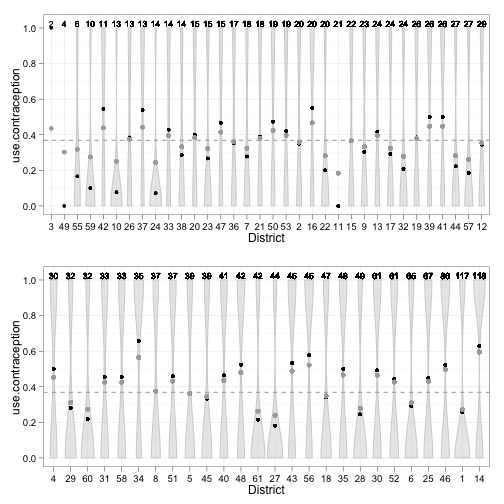
\includegraphics{compare-plot} \end{kframe}}
\end{knitrout}


The figures above show distributions of contraception use for each district (grey violin plots in backgroun) along with point estimates from mixed and fixed-effects only models. The estimates from mixed model (gray dots) are biased toward the group mean (dashed line), relative to estimates from fixed effects model (black dots).
The number of respondents per district are listed at the top of the plot, and districts are ordered by this number (left to right ascending).

The mixed effect and fixed effect estimates disagree most in districts with low numbers of respondents where responses are skewed relative to the overall mean. 
This effect occurs across the whole data set, and is most obvious in districts with very few respondents, and whose cluster mean is very far from the overall mean. 
For example districts 3, 11, and 49 show no variation in responses and the largest disagreements between mixed and random estimates. 
There are also large differences in districts with relatively few, but very skewed responses, e.g. district 10 (n=13), 24 (n=14), or 59 (n=10).
Even in relatively large districts, when responses are very skewed, the mixed and fixed models differ quite a bit e.g. 56 (n=45) and 34 (n=35), which are both above median.



\subsubsection*{urbanness (b)}

I now turn to the effect of living in an urban location on contraceptive use. 
My armchair sociological intuition suggests women living in urban areas will be more likely to use contraception.

I model contraception use as a binomial outcome predicted by the catgorical variable {\tt urban}. 
In addition, I allow the overall prevalence (random slope intercept) and effect of urbanness (random slope) to vary by district.

\begin{knitrout}
\definecolor{shadecolor}{rgb}{.97, .97, .97}{\color{fgcolor}\begin{kframe}
\begin{flushleft}
\ttfamily\noindent
\hlsymbol{m3}{\ }\hlassignement{\usebox{\hlnormalsizeboxlessthan}-}{\ }\hlfunctioncall{glmm}\hlkeyword{(}\hlsymbol{use.contraception}{\ }\hlkeyword{\urltilda{}}{\ }\hlsymbol{urban}{\ }\hlkeyword{+}{\ }\hlkeyword{(}\hlsymbol{urban}{\ }\hlkeyword{+}{\ }\hlnumber{1}{\ }\hlkeyword{|}{\ }\hlsymbol{district}\hlkeyword{)}\hlkeyword{,}\hspace*{\fill}\\
\hlstd{}{\ }{\ }{\ }{\ }\hlargument{data}{\ }\hlargument{=}{\ }\hlsymbol{d}\hlkeyword{,}{\ }\hlargument{family}{\ }\hlargument{=}{\ }\hlsymbol{binomial}\hlkeyword{)}\hspace*{\fill}\\
\hlstd{}\hlfunctioncall{precis}\hlkeyword{(}\hlsymbol{m3}\hlkeyword{)}\mbox{}
\normalfont
\end{flushleft}
\begin{verbatim}
##                        Estimate Std. Error    2.5%   97.5%
## (Intercept)             -0.7178     0.1015 -0.9168 -0.5188
## urban                    0.7412     0.1647  0.4184  1.0639
## ((Intercept)|district)   0.5940         NA      NA      NA
## (urban|district)         0.8163         NA      NA      NA
\end{verbatim}
\begin{flushleft}
\ttfamily\noindent
\hlfunctioncall{show}\hlkeyword{(}\hlsymbol{m3}\hlkeyword{)}\mbox{}
\normalfont
\end{flushleft}
\begin{verbatim}
## Generalized linear mixed model fit by the Laplace approximation 
## Formula: ..1 
##    Data: ..2 
##   AIC  BIC logLik deviance
##  2497 2525  -1243     2487
## Random effects:
##  Groups   Name        Variance Std.Dev. Corr   
##  district (Intercept) 0.353    0.594           
##           urban       0.666    0.816    -0.817 
## Number of obs: 1934, groups: district, 60
## 
## Fixed effects:
##             Estimate Std. Error z value Pr(>|z|)    
## (Intercept)   -0.718      0.102   -7.07  1.6e-12 ***
## urban          0.741      0.165    4.50  6.8e-06 ***
## ---
## Signif. codes:  0 '***' 0.001 '**' 0.01 '*' 0.05 '.' 0.1 ' ' 1 
## 
## Correlation of Fixed Effects:
##       (Intr)
## urban -0.662
\end{verbatim}
\begin{flushleft}
\ttfamily\noindent
\hspace*{\fill}\\
\hlstd{}\hlsymbol{d.re}{\ }\hlassignement{\usebox{\hlnormalsizeboxlessthan}-}{\ }\hlfunctioncall{ranef}\hlkeyword{(}\hlsymbol{m3}\hlkeyword{)}\hlkeyword{\usebox{\hlnormalsizeboxdollar}}\hlsymbol{district}\hspace*{\fill}\\
\hlstd{}\hlsymbol{d.re}\hlkeyword{\usebox{\hlnormalsizeboxdollar}}\hlsymbol{district}{\ }\hlassignement{\usebox{\hlnormalsizeboxlessthan}-}{\ }\hlfunctioncall{as.numeric}\hlkeyword{(}\hlfunctioncall{row.names}\hlkeyword{(}\hlsymbol{d.re}\hlkeyword{)}\hlkeyword{)}\hspace*{\fill}\\
\hlstd{}\hspace*{\fill}\\
\hlstd{}\hlsymbol{g8}{\ }\hlassignement{\usebox{\hlnormalsizeboxlessthan}-}{\ }\hlfunctioncall{ggplot}\hlkeyword{(}\hlsymbol{d.re}\hlkeyword{)}{\ }\hlkeyword{+}{\ }\hlfunctioncall{theme\usebox{\hlnormalsizeboxunderscore}bw}\hlkeyword{(}\hlkeyword{)}\hspace*{\fill}\\
\hlstd{}\hlsymbol{g8}{\ }\hlassignement{\usebox{\hlnormalsizeboxlessthan}-}{\ }\hlsymbol{g8}{\ }\hlkeyword{+}{\ }\hlfunctioncall{geom\usebox{\hlnormalsizeboxunderscore}point}\hlkeyword{(}\hlfunctioncall{aes}\hlkeyword{(}\hlsymbol{\usebox{\hlnormalsizeboxbacktick}(Intercept)\usebox{\hlnormalsizeboxbacktick}}\hlkeyword{,}{\ }\hlsymbol{urban}\hlkeyword{)}\hlkeyword{)}\hspace*{\fill}\\
\hlstd{}\hspace*{\fill}\\
\hlstd{}\hlsymbol{g9}{\ }\hlassignement{\usebox{\hlnormalsizeboxlessthan}-}{\ }\hlfunctioncall{ggplot}\hlkeyword{(}\hlfunctioncall{melt}\hlkeyword{(}\hlsymbol{d.re}\hlkeyword{,}{\ }\hlargument{id.vars}{\ }\hlargument{=}{\ }\hlstring{"district"}\hlkeyword{)}\hlkeyword{)}{\ }\hlkeyword{+}{\ }\hlfunctioncall{theme\usebox{\hlnormalsizeboxunderscore}bw}\hlkeyword{(}\hlkeyword{)}\hspace*{\fill}\\
\hlstd{}\hlsymbol{g9}{\ }\hlassignement{\usebox{\hlnormalsizeboxlessthan}-}{\ }\hlsymbol{g9}{\ }\hlkeyword{+}{\ }\hlfunctioncall{geom\usebox{\hlnormalsizeboxunderscore}line}\hlkeyword{(}\hlfunctioncall{aes}\hlkeyword{(}\hlsymbol{district}\hlkeyword{,}{\ }\hlsymbol{value}\hlkeyword{,}{\ }\hlargument{color}{\ }\hlargument{=}{\ }\hlsymbol{variable}\hlkeyword{)}\hlkeyword{)}{\ }\hlkeyword{+}\hspace*{\fill}\\
\hlstd{}{\ }{\ }{\ }{\ }\hlfunctioncall{scale\usebox{\hlnormalsizeboxunderscore}color\usebox{\hlnormalsizeboxunderscore}grey}\hlkeyword{(}\hlkeyword{)}{\ }\hlkeyword{+}{\ }\hlfunctioncall{ylab}\hlkeyword{(}\hlstring{"varying{\ }effect{\ }estimate"}\hlkeyword{)}\hspace*{\fill}\\
\hlstd{}\hspace*{\fill}\\
\hlstd{}\hlsymbol{a\usebox{\hlnormalsizeboxunderscore}dist}{\ }\hlassignement{\usebox{\hlnormalsizeboxlessthan}-}{\ }\hlfunctioncall{ranef}\hlkeyword{(}\hlsymbol{m3}\hlkeyword{)}\hlkeyword{\usebox{\hlnormalsizeboxdollar}}\hlsymbol{district}\hlkeyword{[}\hlkeyword{,}{\ }\hlnumber{1}\hlkeyword{]}\hspace*{\fill}\\
\hlstd{}\hlsymbol{b\usebox{\hlnormalsizeboxunderscore}dist}{\ }\hlassignement{\usebox{\hlnormalsizeboxlessthan}-}{\ }\hlfunctioncall{ranef}\hlkeyword{(}\hlsymbol{m3}\hlkeyword{)}\hlkeyword{\usebox{\hlnormalsizeboxdollar}}\hlsymbol{district}\hlkeyword{[}\hlkeyword{,}{\ }\hlnumber{2}\hlkeyword{]}\hspace*{\fill}\\
\hlstd{}\hlsymbol{a}{\ }\hlassignement{\usebox{\hlnormalsizeboxlessthan}-}{\ }\hlfunctioncall{fixef}\hlkeyword{(}\hlsymbol{m3}\hlkeyword{)}\hlkeyword{[}\hlnumber{1}\hlkeyword{]}\hspace*{\fill}\\
\hlstd{}\hlsymbol{b}{\ }\hlassignement{\usebox{\hlnormalsizeboxlessthan}-}{\ }\hlfunctioncall{fixef}\hlkeyword{(}\hlsymbol{m3}\hlkeyword{)}\hlkeyword{[}\hlnumber{2}\hlkeyword{]}\hspace*{\fill}\\
\hlstd{}\hlsymbol{urban}{\ }\hlassignement{\usebox{\hlnormalsizeboxlessthan}-}{\ }\hlfunctioncall{logistic}\hlkeyword{(}\hlsymbol{a}{\ }\hlkeyword{+}{\ }\hlsymbol{a\usebox{\hlnormalsizeboxunderscore}dist}{\ }\hlkeyword{+}{\ }\hlsymbol{b\usebox{\hlnormalsizeboxunderscore}dist}{\ }\hlkeyword{+}{\ }\hlsymbol{b}\hlkeyword{)}\hspace*{\fill}\\
\hlstd{}\hlsymbol{rural}{\ }\hlassignement{\usebox{\hlnormalsizeboxlessthan}-}{\ }\hlfunctioncall{logistic}\hlkeyword{(}\hlsymbol{a}{\ }\hlkeyword{+}{\ }\hlsymbol{a\usebox{\hlnormalsizeboxunderscore}dist}\hlkeyword{)}\hspace*{\fill}\\
\hlstd{}\hlsymbol{p.corr}{\ }\hlassignement{\usebox{\hlnormalsizeboxlessthan}-}{\ }\hlfunctioncall{data.frame}\hlkeyword{(}\hlargument{urban}{\ }\hlargument{=}{\ }\hlsymbol{urban}\hlkeyword{,}{\ }\hlargument{rural}{\ }\hlargument{=}{\ }\hlsymbol{rural}\hlkeyword{)}\hspace*{\fill}\\
\hlstd{}\hlsymbol{p.corr}\hlkeyword{\usebox{\hlnormalsizeboxdollar}}\hlsymbol{lab}{\ }\hlassignement{\usebox{\hlnormalsizeboxlessthan}-}{\ }\hlfunctioncall{as.character}\hlkeyword{(}\hlfunctioncall{unique}\hlkeyword{(}\hlsymbol{d}\hlkeyword{\usebox{\hlnormalsizeboxdollar}}\hlsymbol{district}\hlkeyword{)}\hlkeyword{)}\hspace*{\fill}\\
\hlstd{}\hspace*{\fill}\\
\hlstd{}\hlsymbol{g7}{\ }\hlassignement{\usebox{\hlnormalsizeboxlessthan}-}{\ }\hlfunctioncall{ggplot}\hlkeyword{(}\hlsymbol{p.corr}\hlkeyword{)}{\ }\hlkeyword{+}{\ }\hlfunctioncall{theme\usebox{\hlnormalsizeboxunderscore}bw}\hlkeyword{(}\hlkeyword{)}\hspace*{\fill}\\
\hlstd{}\hlsymbol{g7}{\ }\hlassignement{\usebox{\hlnormalsizeboxlessthan}-}{\ }\hlsymbol{g7}{\ }\hlkeyword{+}{\ }\hlfunctioncall{geom\usebox{\hlnormalsizeboxunderscore}abline}\hlkeyword{(}\hlargument{intercept}{\ }\hlargument{=}{\ }\hlnumber{0}\hlkeyword{,}{\ }\hlargument{slope}{\ }\hlargument{=}{\ }\hlnumber{1}\hlkeyword{,}{\ }\hlargument{color}{\ }\hlargument{=}{\ }\hlstring{"grey"}\hlkeyword{)}{\ }\hlkeyword{+}\hspace*{\fill}\\
\hlstd{}{\ }{\ }{\ }{\ }\hlfunctioncall{geom\usebox{\hlnormalsizeboxunderscore}point}\hlkeyword{(}\hlfunctioncall{aes}\hlkeyword{(}\hlsymbol{rural}\hlkeyword{,}{\ }\hlsymbol{urban}\hlkeyword{)}\hlkeyword{)}{\ }\hlkeyword{+}{\ }\hlfunctioncall{xlab}\hlkeyword{(}\hlstring{"prob{\ }contraceptive{\ }use{\ }|{\ }rural"}\hlkeyword{)}{\ }\hlkeyword{+}\hspace*{\fill}\\
\hlstd{}{\ }{\ }{\ }{\ }\hlfunctioncall{ylab}\hlkeyword{(}\hlstring{"prob{\ }contraceptive{\ }use{\ }|{\ }urban"}\hlkeyword{)}{\ }\hlkeyword{+}{\ }\hlfunctioncall{ylim}\hlkeyword{(}\hlfunctioncall{c}\hlkeyword{(}\hlnumber{0}\hlkeyword{,}{\ }\hlnumber{1}\hlkeyword{)}\hlkeyword{)}{\ }\hlkeyword{+}{\ }\hlfunctioncall{xlim}\hlkeyword{(}\hlfunctioncall{c}\hlkeyword{(}\hlnumber{0}\hlkeyword{,}\hspace*{\fill}\\
\hlstd{}{\ }{\ }{\ }{\ }\hlnumber{1}\hlkeyword{)}\hlkeyword{)}\hspace*{\fill}\\
\hlstd{}\hspace*{\fill}\\
\hlstd{}\hlfunctioncall{grid.arrange}\hlkeyword{(}\hlsymbol{g8}\hlkeyword{,}{\ }\hlsymbol{g9}\hlkeyword{,}{\ }\hlsymbol{g7}\hlkeyword{,}{\ }\hlargument{ncol}{\ }\hlargument{=}{\ }\hlnumber{2}\hlkeyword{)}\mbox{}
\normalfont
\end{flushleft}
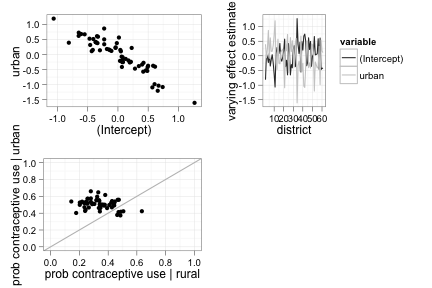
\includegraphics{urban-model} \begin{flushleft}
\ttfamily\noindent
\hspace*{\fill}\\
\hlstd{}\hlfunctioncall{xtabs}\hlkeyword{(}\hlkeyword{\urltilda{}}\hlsymbol{urban}{\ }\hlkeyword{+}{\ }\hlsymbol{district}\hlkeyword{,}{\ }\hlargument{data}{\ }\hlargument{=}{\ }\hlsymbol{d2}\hlkeyword{)}\mbox{}
\normalfont
\end{flushleft}
\begin{verbatim}
##      district
## urban   1   2   3   4   5   6   7   8   9  10  11  12  13  14  15  16  17  18  19  20  21
##     0  54  20   0  19  37  58  18  35  20  13  21  23  16  17  14  18  24  33  22  15  10
##     1  63   0   2  11   2   7   0   2   3   0   0   6   8 101   8   2   0  14   4   0   8
##      district
## urban  22  23  24  25  26  27  28  29  30  31  32  33  34  35  36  37  38  39  40  41  42
##     0  20  15  14  49  13  39  45  25  45  27  24   7  26  28  14  13   7  24  12  23   6
##     1   0   0   0  18   0   5   4   7  16   6   0   7   9  20   3   0   7   2  29   3   5
##      district
## urban  43  44  45  46  47  48  49  50  51  52  53  55  56  57  58  59  60  61
##     0  28  27  34  74   9  26   4  15  20  42   0   0  24  23  20  10  22  31
##     1  17   0   5  12   6  16   0   4  17  19  19   6  21   4  13   0  10  11
\end{verbatim}
\end{kframe}}
\end{knitrout}


The fit estimated a negative correlation between the varying intercepts and slopes on urban, per district:  $\rho = - 0. 662$. 
This correlation is shown in figures above (top row), which depict the coefficients plotted against one another (left panel) and by district (right panel).

As indicated by the figures, the correlation implies a tradeoff between these two coefficients, i.e. the differences between districts were such that they had {\em either} high contraceptive use overall (positive intercept effect) or a strong effect of urbanness (positive slope effect). 
This points to an interaction of sorts, where urbanness has a positive effect on contraceptive use in districts with low contraceptive use overall, but the effect of urbanness is negative in districts with high contraception use.

This effect is shown in the bottom figure, which plots the predicted probability of contraception use for an urban resident of a district against that predicted for a rural resident in the same district. 

\subsection*{Oxford boy growth}

Now, I model the heights of boys measured at different ages. 

\begin{knitrout}
\definecolor{shadecolor}{rgb}{.97, .97, .97}{\color{fgcolor}\begin{kframe}
\begin{flushleft}
\ttfamily\noindent
\hlsymbol{d3}{\ }\hlassignement{\usebox{\hlnormalsizeboxlessthan}-}{\ }\hlfunctioncall{read.csv}\hlkeyword{(}\hlstring{"Oxboys.csv"}\hlkeyword{)}\hspace*{\fill}\\
\hlstd{}\hlfunctioncall{head}\hlkeyword{(}\hlsymbol{d3}\hlkeyword{,}{\ }\hlargument{n}{\ }\hlargument{=}{\ }\hlnumber{1}\hlkeyword{)}\mbox{}
\normalfont
\end{flushleft}
\begin{verbatim}
##   Subject age height Occasion
## 1       1  -1  140.5        1
\end{verbatim}
\end{kframe}}
\end{knitrout}


The data include several boys ({\tt Subject}) that have ({\tt height}) measured over time ({\tt Age}). 

\begin{knitrout}
\definecolor{shadecolor}{rgb}{.97, .97, .97}{\color{fgcolor}\begin{kframe}
\begin{flushleft}
\ttfamily\noindent
\hlcomment{\usebox{\hlnormalsizeboxhash}reorder{\ }by{\ }intercept}\hspace*{\fill}\\
\hlstd{}\hlsymbol{d3}{\ }\hlassignement{\usebox{\hlnormalsizeboxlessthan}-}{\ }\hlfunctioncall{within}\hlkeyword{(}\hlsymbol{d3}\hlkeyword{,}{\ }\hlsymbol{Subject}{\ }\hlassignement{\usebox{\hlnormalsizeboxlessthan}-}{\ }\hlfunctioncall{as.factor}\hlkeyword{(}\hlsymbol{Subject}\hlkeyword{)}\hlkeyword{)}\hspace*{\fill}\\
\hlstd{}\hlsymbol{d3}{\ }\hlassignement{\usebox{\hlnormalsizeboxlessthan}-}{\ }\hlfunctioncall{within}\hlkeyword{(}\hlsymbol{d3}\hlkeyword{,}{\ }\hlsymbol{Subject}{\ }\hlassignement{\usebox{\hlnormalsizeboxlessthan}-}{\ }\hlfunctioncall{factor}\hlkeyword{(}\hlsymbol{Subject}\hlkeyword{,}{\ }\hlargument{levels}{\ }\hlargument{=}{\ }\hlfunctioncall{order}\hlkeyword{(}\hlfunctioncall{with}\hlkeyword{(}\hlsymbol{d3}\hlkeyword{,}\hspace*{\fill}\\
\hlstd{}{\ }{\ }{\ }{\ }\hlfunctioncall{by}\hlkeyword{(}\hlsymbol{height}\hlkeyword{,}{\ }\hlsymbol{Subject}\hlkeyword{,}{\ }\hlsymbol{min}\hlkeyword{)}\hlkeyword{)}\hlkeyword{)}\hlkeyword{)}\hlkeyword{)}\hspace*{\fill}\\
\hlstd{}\hspace*{\fill}\\
\hlstd{}\hlsymbol{g3}{\ }\hlassignement{\usebox{\hlnormalsizeboxlessthan}-}{\ }\hlfunctioncall{ggplot}\hlkeyword{(}\hlsymbol{d3}\hlkeyword{)}\hspace*{\fill}\\
\hlstd{}\hlfunctioncall{grid.arrange}\hlkeyword{(}\hlsymbol{g3}{\ }\hlkeyword{+}{\ }\hlfunctioncall{geom\usebox{\hlnormalsizeboxunderscore}point}\hlkeyword{(}\hlfunctioncall{aes}\hlkeyword{(}\hlsymbol{age}\hlkeyword{,}{\ }\hlsymbol{height}\hlkeyword{)}\hlkeyword{)}{\ }\hlkeyword{+}{\ }\hlfunctioncall{facet\usebox{\hlnormalsizeboxunderscore}wrap}\hlkeyword{(}\hlkeyword{\urltilda{}}\hlsymbol{Subject}\hlkeyword{)}\hlkeyword{,}\hspace*{\fill}\\
\hlstd{}{\ }{\ }{\ }{\ }\hlsymbol{g3}{\ }\hlkeyword{+}{\ }\hlfunctioncall{geom\usebox{\hlnormalsizeboxunderscore}point}\hlkeyword{(}\hlfunctioncall{aes}\hlkeyword{(}\hlsymbol{age}\hlkeyword{,}{\ }\hlsymbol{height}\hlkeyword{,}{\ }\hlargument{size}{\ }\hlargument{=}{\ }\hlsymbol{Subject}\hlkeyword{)}\hlkeyword{)}{\ }\hlkeyword{+}{\ }\hlfunctioncall{opts}\hlkeyword{(}\hlargument{legend.position}{\ }\hlargument{=}{\ }\hlstring{"none"}\hlkeyword{)}\hlkeyword{,}\hspace*{\fill}\\
\hlstd{}{\ }{\ }{\ }{\ }\hlargument{ncol}{\ }\hlargument{=}{\ }\hlnumber{1}\hlkeyword{)}\mbox{}
\normalfont
\end{flushleft}
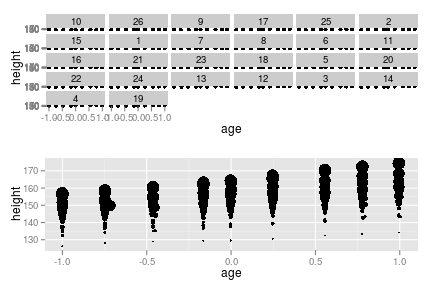
\includegraphics{plot-ox} \end{kframe}}
\end{knitrout}


The top figure is a panel plot of each subject. 
The bottom figure shows all data plotted on one figure, but with a different dot size for each subject. 


The data look relatively linear. As these are growing boys, for now, it makes sense to model height as a Normal random variable predicted by {\tt age}. 
Note that this formulation ignores the autocorrelation we expect from a time series.

\subsubsection*{individual level effects (a)}

I model height $h_{ij}$ the height observed in {\tt Subject} $j$ at age $i$
\begin{align*}
&h_{ij} \sim {\rm Normal}(\mu_{ij}, \sigma)\\
&\mu_{ij} = \alpha + \alpha_j + (\beta + \beta_j){\rm age}_i\\
&\left( \begin{matrix}\alpha_j\\ \beta_j\end{matrix}\right) \sim {\rm Normal}
\left [ \left( \begin{matrix}0\\ 0\end{matrix}\right), \left( \begin{matrix}\sigma^2_\alpha & \sigma_\alpha \sigma_\beta \rho\\ \sigma_\alpha \sigma_\beta \rho &\sigma^2_\beta\end{matrix}\right)\right]
\end{align*}

\begin{knitrout}
\definecolor{shadecolor}{rgb}{.97, .97, .97}{\color{fgcolor}\begin{kframe}
\begin{flushleft}
\ttfamily\noindent
\hspace*{\fill}\\
\hlstd{}\hlsymbol{m4}{\ }\hlassignement{\usebox{\hlnormalsizeboxlessthan}-}{\ }\hlfunctioncall{lmer}\hlkeyword{(}\hlsymbol{height}{\ }\hlkeyword{\urltilda{}}{\ }\hlsymbol{age}{\ }\hlkeyword{+}{\ }\hlkeyword{(}\hlsymbol{age}{\ }\hlkeyword{|}{\ }\hlsymbol{Subject}\hlkeyword{)}\hlkeyword{,}{\ }\hlargument{data}{\ }\hlargument{=}{\ }\hlsymbol{d3}\hlkeyword{)}\hspace*{\fill}\\
\hlstd{}\hlfunctioncall{precis}\hlkeyword{(}\hlsymbol{m4}\hlkeyword{)}\mbox{}
\normalfont
\end{flushleft}
\begin{verbatim}
##                       Estimate Std. Error    2.5%   97.5%
## (Intercept)           149.3718     1.5854 146.264 152.479
## age                     6.5255     0.3363   5.866   7.185
## ((Intercept)|Subject)   8.0811         NA      NA      NA
## (age|Subject)           1.6807         NA      NA      NA
## (Residual)              0.6599         NA      NA      NA
\end{verbatim}
\begin{flushleft}
\ttfamily\noindent
\hspace*{\fill}\\
\hlstd{}\hlfunctioncall{sd}\hlkeyword{(}\hlfunctioncall{ranef}\hlkeyword{(}\hlsymbol{m4}\hlkeyword{)}\hlkeyword{\usebox{\hlnormalsizeboxdollar}}\hlsymbol{Subject}\hlkeyword{[}\hlkeyword{,}{\ }\hlnumber{1}\hlkeyword{]}\hlkeyword{)}{\ }{\ }\hlcomment{\usebox{\hlnormalsizeboxhash}\usebox{\hlnormalsizeboxhash}{\ }sample{\ }standard{\ }deviation{\ }in{\ }estimated{\ }random{\ }intercept{\ }effects}\mbox{}
\normalfont
\end{flushleft}
\begin{verbatim}
## [1] 8.078
\end{verbatim}
\begin{flushleft}
\ttfamily\noindent
\hlfunctioncall{sd}\hlkeyword{(}\hlfunctioncall{ranef}\hlkeyword{(}\hlsymbol{m4}\hlkeyword{)}\hlkeyword{\usebox{\hlnormalsizeboxdollar}}\hlsymbol{Subject}\hlkeyword{[}\hlkeyword{,}{\ }\hlnumber{2}\hlkeyword{]}\hlkeyword{)}{\ }{\ }\hlcomment{\usebox{\hlnormalsizeboxhash}\usebox{\hlnormalsizeboxhash}{\ }sample{\ }standard{\ }deviation{\ }in{\ }estimated{\ }random{\ }slope{\ }effect}\mbox{}
\normalfont
\end{flushleft}
\begin{verbatim}
## [1] 1.648
\end{verbatim}
\end{kframe}}
\end{knitrout}


The estimate for the Subject random intercept on height is much higher than that of the Subject$\times$age effect. 
Further the variance of the estimated random intercept is much larger than that of random slope on age. 

This implies that per-subject variation, unrelated to age, explains more variation than per-subject variation that is related to age.

\subsubsection*{individual level effects (b)}

\begin{knitrout}
\definecolor{shadecolor}{rgb}{.97, .97, .97}{\color{fgcolor}\begin{kframe}
\begin{flushleft}
\ttfamily\noindent
\hlsymbol{s.m4}{\ }\hlassignement{\usebox{\hlnormalsizeboxlessthan}-}{\ }\hlfunctioncall{summary}\hlkeyword{(}\hlsymbol{m4}\hlkeyword{)}\hspace*{\fill}\\
\hlstd{}\hlsymbol{s.m4}\mbox{}
\normalfont
\end{flushleft}
\begin{verbatim}
## Linear mixed model fit by REML 
## Formula: height ~ age + (age | Subject) 
##    Data: d3 
##  AIC BIC logLik deviance REMLdev
##  736 757   -362      726     724
## Random effects:
##  Groups   Name        Variance Std.Dev. Corr  
##  Subject  (Intercept) 65.304   8.08           
##           age          2.825   1.68     0.641 
##  Residual              0.435   0.66           
## Number of obs: 234, groups: Subject, 26
## 
## Fixed effects:
##             Estimate Std. Error t value
## (Intercept)  149.372      1.585    94.2
## age            6.525      0.336    19.4
## 
## Correlation of Fixed Effects:
##     (Intr)
## age 0.628 
\end{verbatim}
\end{kframe}}
\end{knitrout}


There is a positive correlation between random intercept and slope (on age) effects of subject. 
This relationship is noisy (plot not shown).
It makes sense mechanistically that the boys who are bigger in general durign the study, also grew faster over the ages at which they were observed. 
Boys who grew fast prior to the study would tend to be larger upon initiation of the study, and one might expect these same boys to continue to grow faster. 
In a sense this correlation captures some of our intution that this is a {\em time series}.

Now, I'll predict observed heights assuming we're sampling a new set of boys from the same population, across the same ages sampled. 

\subsubsection*{individual level effects (b)}

To simulate new boys, we need to construct random draws from a normal distribution centered on zero, but with variance-covariance structure given by 
\[
\left(\begin{matrix}\sigma^2_\alpha & \sigma_\alpha \sigma_\beta \rho\\ \sigma_\alpha \sigma_\beta \rho &\sigma^2_\beta\end{matrix}\right).
\]
We can then predict heights from our model above, using these simulated varying effects. 
The function {\tt VarCorr} gives this matrix for our model.
\begin{knitrout}
\definecolor{shadecolor}{rgb}{.97, .97, .97}{\color{fgcolor}\begin{kframe}
\begin{flushleft}
\ttfamily\noindent
\hlsymbol{VC}{\ }\hlassignement{\usebox{\hlnormalsizeboxlessthan}-}{\ }\hlfunctioncall{VarCorr}\hlkeyword{(}\hlsymbol{m4}\hlkeyword{)}\hlkeyword{\usebox{\hlnormalsizeboxdollar}}\hlsymbol{Subject}\hspace*{\fill}\\
\hlstd{}\hlfunctioncall{attr}\hlkeyword{(}\hlsymbol{VC}\hlkeyword{,}{\ }\hlstring{"stddev"}\hlkeyword{)}{\ }{\ }\hlcomment{\usebox{\hlnormalsizeboxhash}{\ }random{\ }effects{\ }standard{\ }deviations}\mbox{}
\normalfont
\end{flushleft}
\begin{verbatim}
## (Intercept)         age 
##       8.081       1.681 
\end{verbatim}
\begin{flushleft}
\ttfamily\noindent
\hlfunctioncall{attr}\hlkeyword{(}\hlsymbol{VC}\hlkeyword{,}{\ }\hlstring{"correlation"}\hlkeyword{)}{\ }{\ }\hlcomment{\usebox{\hlnormalsizeboxhash}{\ }random{\ }effects{\ }correlatins}\mbox{}
\normalfont
\end{flushleft}
\begin{verbatim}
##             (Intercept)    age
## (Intercept)      1.0000 0.6413
## age              0.6413 1.0000
\end{verbatim}
\begin{flushleft}
\ttfamily\noindent
\hlcomment{\usebox{\hlnormalsizeboxhash}S{\ }\usebox{\hlnormalsizeboxlessthan}-{\ }matrix({\ }c({\ }sa\usebox{\hlnormalsizeboxhat}2{\ },{\ }sa*sb*rho{\ },{\ }sa*sb*rho{\ },{\ }sb\usebox{\hlnormalsizeboxhat}2{\ }){\ },{\ }nrow=2{\ })}\mbox{}
\normalfont
\end{flushleft}
\end{kframe}}
\end{knitrout}

Note that we could also construct it directly as in the commented-out line using the random effects standard deviations ($\sigma_\alpha, \sigma_\beta$)
and correlation ($\rho$; given by the off diagonal of the correlation matrix) printed above. 

\begin{knitrout}
\definecolor{shadecolor}{rgb}{.97, .97, .97}{\color{fgcolor}\begin{kframe}
\begin{flushleft}
\ttfamily\noindent
\hlsymbol{VC}{\ }\hlassignement{\usebox{\hlnormalsizeboxlessthan}-}{\ }\hlfunctioncall{VarCorr}\hlkeyword{(}\hlsymbol{m4}\hlkeyword{)}\hlkeyword{\usebox{\hlnormalsizeboxdollar}}\hlsymbol{Subject}\hspace*{\fill}\\
\hlstd{}\hlfunctioncall{attr}\hlkeyword{(}\hlsymbol{VC}\hlkeyword{,}{\ }\hlstring{"stddev"}\hlkeyword{)}{\ }{\ }\hlcomment{\usebox{\hlnormalsizeboxhash}{\ }random{\ }effects{\ }standard{\ }deviations}\mbox{}
\normalfont
\end{flushleft}
\begin{verbatim}
## (Intercept)         age 
##       8.081       1.681 
\end{verbatim}
\begin{flushleft}
\ttfamily\noindent
\hlfunctioncall{attr}\hlkeyword{(}\hlsymbol{VC}\hlkeyword{,}{\ }\hlstring{"correlation"}\hlkeyword{)}{\ }{\ }\hlcomment{\usebox{\hlnormalsizeboxhash}{\ }random{\ }effects{\ }correlatins}\mbox{}
\normalfont
\end{flushleft}
\begin{verbatim}
##             (Intercept)    age
## (Intercept)      1.0000 0.6413
## age              0.6413 1.0000
\end{verbatim}
\begin{flushleft}
\ttfamily\noindent
\hlcomment{\usebox{\hlnormalsizeboxhash}S{\ }\usebox{\hlnormalsizeboxlessthan}-{\ }matrix({\ }c({\ }sa\usebox{\hlnormalsizeboxhat}2{\ },{\ }sa*sb*rho{\ },{\ }sa*sb*rho{\ },{\ }sb\usebox{\hlnormalsizeboxhat}2{\ }){\ },{\ }nrow=2{\ })}\hspace*{\fill}\\
\hlstd{}\hspace*{\fill}\\
\hlstd{}\hlfunctioncall{set.seed}\hlkeyword{(}\hlnumber{10}\hlkeyword{)}\hspace*{\fill}\\
\hlstd{}\hlsymbol{ages}{\ }\hlassignement{\usebox{\hlnormalsizeboxlessthan}-}{\ }\hlfunctioncall{unique}\hlkeyword{(}\hlsymbol{d3}\hlkeyword{\usebox{\hlnormalsizeboxdollar}}\hlsymbol{age}\hlkeyword{)}\hspace*{\fill}\\
\hlstd{}\hlsymbol{NREP}{\ }\hlassignement{\usebox{\hlnormalsizeboxlessthan}-}{\ }\hlnumber{10}\hspace*{\fill}\\
\hlstd{}\hlsymbol{re.pred}{\ }\hlassignement{\usebox{\hlnormalsizeboxlessthan}-}{\ }\hlfunctioncall{mvrnorm}\hlkeyword{(}\hlsymbol{NREP}\hlkeyword{,}{\ }\hlargument{mu}{\ }\hlargument{=}{\ }\hlfunctioncall{c}\hlkeyword{(}\hlnumber{0}\hlkeyword{,}{\ }\hlnumber{0}\hlkeyword{)}\hlkeyword{,}{\ }\hlargument{Sigma}{\ }\hlargument{=}{\ }\hlsymbol{VC}\hlkeyword{)}\hspace*{\fill}\\
\hlstd{}\hlsymbol{a}{\ }\hlassignement{\usebox{\hlnormalsizeboxlessthan}-}{\ }\hlfunctioncall{fixef}\hlkeyword{(}\hlsymbol{m4}\hlkeyword{)}\hlkeyword{[}\hlstring{"(Intercept)"}\hlkeyword{]}\hspace*{\fill}\\
\hlstd{}\hlsymbol{b}{\ }\hlassignement{\usebox{\hlnormalsizeboxlessthan}-}{\ }\hlfunctioncall{fixef}\hlkeyword{(}\hlsymbol{m4}\hlkeyword{)}\hlkeyword{[}\hlstring{"age"}\hlkeyword{]}\hspace*{\fill}\\
\hlstd{}\hlsymbol{height.pred}{\ }\hlassignement{\usebox{\hlnormalsizeboxlessthan}-}{\ }\hlfunctioncall{sapply}\hlkeyword{(}\hlsymbol{ages}\hlkeyword{,}{\ }\hlkeyword{function}\hlkeyword{(}\hlformalargs{x}\hlkeyword{)}{\ }\hlsymbol{a}{\ }\hlkeyword{+}{\ }\hlsymbol{re.pred}\hlkeyword{[}\hlkeyword{,}{\ }\hlstring{"(Intercept)"}\hlkeyword{]}{\ }\hlkeyword{+}\hspace*{\fill}\\
\hlstd{}{\ }{\ }{\ }{\ }\hlkeyword{(}\hlsymbol{b}{\ }\hlkeyword{+}{\ }\hlsymbol{re.pred}\hlkeyword{[}\hlkeyword{,}{\ }\hlstring{"age"}\hlkeyword{]}\hlkeyword{)}{\ }\hlkeyword{*}{\ }\hlsymbol{x}\hlkeyword{)}\hspace*{\fill}\\
\hlstd{}\hlsymbol{df.prd}{\ }\hlassignement{\usebox{\hlnormalsizeboxlessthan}-}{\ }\hlfunctioncall{as.data.frame}\hlkeyword{(}\hlfunctioncall{t}\hlkeyword{(}\hlsymbol{height.pred}\hlkeyword{)}\hlkeyword{)}\hspace*{\fill}\\
\hlstd{}\hlfunctioncall{names}\hlkeyword{(}\hlsymbol{df.prd}\hlkeyword{)}{\ }\hlassignement{\usebox{\hlnormalsizeboxlessthan}-}{\ }\hlfunctioncall{as.character}\hlkeyword{(}\hlnumber{1}\hlkeyword{:}\hlsymbol{NREP}\hlkeyword{)}\hspace*{\fill}\\
\hlstd{}\hlsymbol{df.prd}\hlkeyword{\usebox{\hlnormalsizeboxdollar}}\hlsymbol{age}{\ }\hlassignement{\usebox{\hlnormalsizeboxlessthan}-}{\ }\hlsymbol{ages}\hspace*{\fill}\\
\hlstd{}\hspace*{\fill}\\
\hlstd{}\hlsymbol{df}{\ }\hlassignement{\usebox{\hlnormalsizeboxlessthan}-}{\ }\hlfunctioncall{melt}\hlkeyword{(}\hlsymbol{df.prd}\hlkeyword{,}{\ }\hlargument{id.vars}{\ }\hlargument{=}{\ }\hlfunctioncall{c}\hlkeyword{(}\hlstring{"age"}\hlkeyword{)}\hlkeyword{)}\hspace*{\fill}\\
\hlstd{}\hlfunctioncall{names}\hlkeyword{(}\hlsymbol{df}\hlkeyword{)}\hlkeyword{[}\hlnumber{2}\hlkeyword{:}\hlnumber{3}\hlkeyword{]}{\ }\hlassignement{\usebox{\hlnormalsizeboxlessthan}-}{\ }\hlfunctioncall{c}\hlkeyword{(}\hlstring{"Subject"}\hlkeyword{,}{\ }\hlstring{"height"}\hlkeyword{)}\hspace*{\fill}\\
\hlstd{}\hlcomment{\usebox{\hlnormalsizeboxhash}reorder{\ }by{\ }intercept}\hspace*{\fill}\\
\hlstd{}\hlsymbol{df}{\ }\hlassignement{\usebox{\hlnormalsizeboxlessthan}-}{\ }\hlfunctioncall{within}\hlkeyword{(}\hlsymbol{df}\hlkeyword{,}{\ }\hlsymbol{Subject}{\ }\hlassignement{\usebox{\hlnormalsizeboxlessthan}-}{\ }\hlfunctioncall{as.factor}\hlkeyword{(}\hlsymbol{Subject}\hlkeyword{)}\hlkeyword{)}\hspace*{\fill}\\
\hlstd{}\hlsymbol{df}{\ }\hlassignement{\usebox{\hlnormalsizeboxlessthan}-}{\ }\hlfunctioncall{within}\hlkeyword{(}\hlsymbol{df}\hlkeyword{,}{\ }\hlsymbol{Subject}{\ }\hlassignement{\usebox{\hlnormalsizeboxlessthan}-}{\ }\hlfunctioncall{factor}\hlkeyword{(}\hlsymbol{Subject}\hlkeyword{,}{\ }\hlargument{levels}{\ }\hlargument{=}{\ }\hlfunctioncall{order}\hlkeyword{(}\hlfunctioncall{with}\hlkeyword{(}\hlsymbol{df}\hlkeyword{,}\hspace*{\fill}\\
\hlstd{}{\ }{\ }{\ }{\ }\hlfunctioncall{by}\hlkeyword{(}\hlsymbol{height}\hlkeyword{,}{\ }\hlsymbol{Subject}\hlkeyword{,}{\ }\hlsymbol{min}\hlkeyword{)}\hlkeyword{)}\hlkeyword{)}\hlkeyword{)}\hlkeyword{)}\hspace*{\fill}\\
\hlstd{}\hspace*{\fill}\\
\hlstd{}\hspace*{\fill}\\
\hlstd{}\hlsymbol{g5}{\ }\hlassignement{\usebox{\hlnormalsizeboxlessthan}-}{\ }\hlfunctioncall{ggplot}\hlkeyword{(}\hlsymbol{df}\hlkeyword{)}\hspace*{\fill}\\
\hlstd{}\hlfunctioncall{grid.arrange}\hlkeyword{(}\hlsymbol{g5}{\ }\hlkeyword{+}{\ }\hlfunctioncall{geom\usebox{\hlnormalsizeboxunderscore}point}\hlkeyword{(}\hlfunctioncall{aes}\hlkeyword{(}\hlsymbol{age}\hlkeyword{,}{\ }\hlsymbol{height}\hlkeyword{,}{\ }\hlargument{size}{\ }\hlargument{=}{\ }\hlsymbol{Subject}\hlkeyword{)}\hlkeyword{)}\hlkeyword{,}\hspace*{\fill}\\
\hlstd{}{\ }{\ }{\ }{\ }\hlsymbol{g5}{\ }\hlkeyword{+}{\ }\hlfunctioncall{geom\usebox{\hlnormalsizeboxunderscore}point}\hlkeyword{(}\hlfunctioncall{aes}\hlkeyword{(}\hlsymbol{age}\hlkeyword{,}{\ }\hlsymbol{height}\hlkeyword{)}\hlkeyword{)}{\ }\hlkeyword{+}{\ }\hlfunctioncall{facet\usebox{\hlnormalsizeboxunderscore}wrap}\hlkeyword{(}\hlkeyword{\urltilda{}}\hlsymbol{Subject}\hlkeyword{)}\hlkeyword{,}{\ }\hlargument{ncol}{\ }\hlargument{=}{\ }\hlnumber{1}\hlkeyword{)}\mbox{}
\normalfont
\end{flushleft}
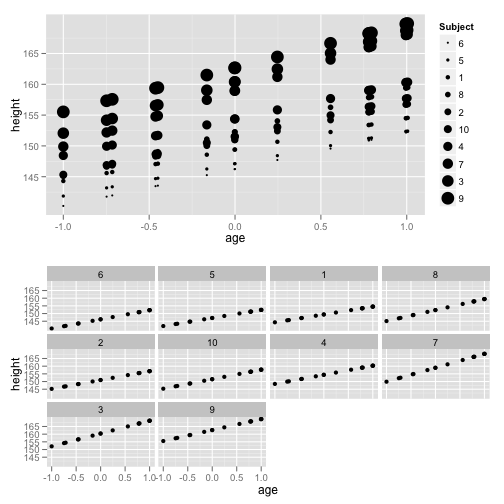
\includegraphics{ox-simulate} \end{kframe}}
\end{knitrout}


The simulated data seem to have similar structure... 


\newpage
\subsection*{Colophon}

\begin{knitrout}
\definecolor{shadecolor}{rgb}{.97, .97, .97}{\color{fgcolor}\begin{kframe}
\begin{flushleft}
\ttfamily\noindent
\hlfunctioncall{require}\hlkeyword{(}\hlsymbol{knitr}\hlkeyword{)}{\ }{\ }\hlcomment{\usebox{\hlnormalsizeboxhash}\usebox{\hlnormalsizeboxhash}\usebox{\hlnormalsizeboxhash}{\ }the{\ }package}\hspace*{\fill}\\
\hlstd{}\hlfunctioncall{knit}\hlkeyword{(}\hlfunctioncall{paste}\hlkeyword{(}\hlfunctioncall{getwd}\hlkeyword{(}\hlkeyword{)}\hlkeyword{,}{\ }\hlstring{"hw9ashander.Rnw"}\hlkeyword{,}{\ }\hlargument{sep}{\ }\hlargument{=}{\ }\hlstring{"/"}\hlkeyword{)}\hlkeyword{)}{\ }{\ }\hlcomment{\usebox{\hlnormalsizeboxhash}\usebox{\hlnormalsizeboxhash}{\ }to{\ }run1}\hspace*{\fill}\\
\hlstd{}\hspace*{\fill}\\
\hlstd{}\hlcomment{\usebox{\hlnormalsizeboxhash}\usebox{\hlnormalsizeboxhash}x{\ }to{\ }use{\ }all{\ }cores}\hspace*{\fill}\\
\hlstd{}\hlfunctioncall{require}\hlkeyword{(}\hlsymbol{snowfall}\hlkeyword{)}\hspace*{\fill}\\
\hlstd{}\hlfunctioncall{sfInit}\hlkeyword{(}\hlargument{parallel}{\ }\hlargument{=}{\ }\hlnumber{TRUE}\hlkeyword{,}{\ }\hlargument{cpus}{\ }\hlargument{=}{\ }\hlnumber{4}\hlkeyword{)}\hspace*{\fill}\\
\hlstd{}\hlfunctioncall{sfLibrary}\hlkeyword{(}\hlsymbol{rethinking}\hlkeyword{)}\hspace*{\fill}\\
\hlstd{}\hlfunctioncall{sfExportAll}\hlkeyword{(}\hlkeyword{)}\hspace*{\fill}\\
\hlstd{}\hlfunctioncall{sfStop}\hlkeyword{(}\hlkeyword{)}\mbox{}
\normalfont
\end{flushleft}
\end{kframe}}
\end{knitrout}


\end{document}
